%X TS-program = pdflatex
% !TEX encoding = UTF-8 Unicode

% This is a simple template for a LaTeX document using the "article" class.
% See "book", "report", "letter" for other types of document.

\documentclass[10pt]{amsart} % use larger type; default would be 10pt
\usepackage{color}
\usepackage[utf8]{inputenc} % set input encoding (not needed with XeLaTeX)

%%% Examples of Article customizations
% These packages are optional, depending whether you want the features they provide.
% See the LaTeX Companion or other references for full information.

%%% PAGE DIMENSIONS

%\usepackage[top=20mm,right=20mm,bottom=15mm,left=20mm]{geometry}
% \geometry{margins=2in} % for example, change the margins to 2 inches all round
% \geometry{landscape} % set up the page for landscape
%   read geometry.pdf for detailed page layout information

\usepackage{graphicx} % support the \includegraphics command and options

% \usepackage[parfill]{parskip} % Activate to begin paragraphs with an empty line rather than an indent

%%% PACKAGES
\usepackage{booktabs} % for much better looking tables
\usepackage{array} % for better arrays (eg matrices) in maths
%\usepackage{paralist} % very flexible & customisable lists (eg. enumerate/itemize, etc.)

%\usepackage{subfig} % make it possible to include more than one captioned figure/table in a single float
\usepackage{amsfonts}
\usepackage{amsthm}
\usepackage{tikz}
\usepackage{amsmath}
\usepackage{float}
\usepackage{graphicx}
\usepackage{caption}
\usepackage{subcaption}
\usepackage{color}
\usepackage{amssymb}
\usepackage{bm}

% These packages are all incorporated in the memoir class to one degree or another...

%%% HEADERS & FOOTERS
%\usepackage{fancyhdr} % This should be set AFTER setting up the page geometry
%\pagestyle{fancy} % options: empty , plain , fancy
%\renewcommand{\headrulewidth}{0pt} % customise the layout...
%\lhead{}\chead{}\rhead{}
%\lfoot{}\cfoot{\thepage}\rfoot{}

%%% SECTION TITLE APPEARANCE
%\usepackage{sectsty}
%\allsectionsfont{\sffamily\mdseries\upshape} % (See the fntguide.pdf for font help)
% (This matches ConTeXt defaults)

%%% ToC (table of contents) APPEARANCE
%\usepackage[nottoc,notlof,notlot]{tocbibind} % Put the bibliography in the ToC
%\usepackage[titles,subfigure]{tocloft} % Alter the style of the Table of Contents
%\renewcommand{\cftsecfont}{\rmfamily\mdseries\upshape}
%\renewcommand{\cftsecpagefont}{\rmfamily\mdseries\upshape} % No bold!


\newtheorem{theorem}{Theorem} 
\newtheorem{lemma}{Lemma}
\newtheorem{propn}{Proposition}
\newtheorem*{thmm}{Theorem}
\newtheorem{remk}{Remark} 
\newtheorem{corol}{Corollary}
\newtheorem{definition}{Definition}



\newtheorem{thm}{Theorem}[section] 
\newtheorem{prop}[thm]{Proposition} 
\newtheorem{lem}[thm]{Lemma}
\newtheorem{cor}[thm]{Corollary} 
\newtheorem{con}[thm]{Conjecture} 

\theoremstyle{definition}
\newtheorem{defn}[thm]{Definition}
\newtheorem*{rem}{Remark}
%\newtheorem*{nota}{Notation}
\newtheorem*{nota}{Notation}
\newtheorem{cla}[thm]{Claim}
\newtheorem{ex}[thm]{Example}
\newtheorem{exs}[thm]{Examples}
\newtheorem*{exer}{Exercise}
\newtheorem{case}{Case}
\newtheorem{conj}{Conjecture}

\definecolor{sotonblue}{rgb}{0.0,0.394,0.597}

\newcommand{\pspace}{$(\Omega_\alpha,\mathcal{F}_\alpha,P_\alpha)$ } 
\DeclareMathOperator{\Aut}{Aut}
\DeclareMathOperator{\Pspace}{(\Omega, \mathcal{F},\mathbb{P})}
\DeclareMathOperator{\Pspacen}{(\Omega_n, \mathcal{F}_n,\mathbb{P}_n)}

\DeclareMathOperator{\T}{\mathcal{T}}
\DeclareMathOperator{\Y}{\mathcal{Y}}
\DeclareMathOperator{\A}{\mathcal{A}}
\DeclareMathOperator{\B}{\mathcal{B}}
\DeclareMathOperator{\F}{\mathcal{F}}
\DeclareMathOperator{\fix}{fix}
\DeclareMathOperator{\N}{\mathbb{N}}
\definecolor{c30a3f9}{RGB}{48,163,249}
\definecolor{c30a3f9}{RGB}{48,163,249}


%opening
 \title{Calculating the expected automorphism group for RRTs}
\author{David Matthews}
\begin{document}
\maketitle

\section{Labeled Trees}

The set, $\tilde{\T}_n$, of rooted, labeled trees on $n$ vertices can be acted on by the subgroup, $S_n$ of the symmetric group that preserves 1 by permuting vertices.  The orbits of this action are the unlabeled rooted trees on $n$ vertices.     

\section{Random recursive trees}


A \emph{random recursive tree} (RRT) is a labelled, rooted tree obtained by assigning a root vertex and adding $n-1$ vertices one by one such that each new vertex is joined by an edge to a randomly and uniformly chosen existing vertex. It is natural to consider RRTs as nested sequences of rooted, labelled trees
\[T_{1} \subset T_{2} \subset \dots \subset T_{n}\]
Each $T_{t}$ has precisely $t$ vertices (and $(t-1)$ edges).  In particular $T_1$ is the labelled rooted tree with one vertex and no edges.  The RRT process proceeds as follows: at time $t$ vertex $v$ is chosen uniformly at random from $V(T_{t-1})$ and a new vertex $v_{t}$ is attached to $T_{t-1}$ via the edge $\{(v,v_{t})\}$. We use the notation $\{T_i\}_{i=1}^{n}$ to mean a RRT on $n$ vertice and we denote the set of all RRTs on $n$ vertices by $\T_n$

Let $T = (V(T),E(T))$ be a labelled tree (not necessarily a RRT) and $d(v,w)$ be the length of the (unique) shortest path between any pair of vertices $v\neq w \in V(T)$.  Every vertex $v \neq 1 $ has a well defined \emph{father}: the unique vertex $v'$ adjacent to $v$ such that $d(v',1)< d(v,1)$.   Let $\N_n = \{1,2,3,\dots,n\}$. 

\begin{lem}
 Let $\mathcal{F}_n$ be the set of functions $f: \N_n \longrightarrow \N_n$ such that $f(1) = 1$ and $f(i) <i$ for $i = 2,3,\dots n$.  There is a bijection between $T_n$ and $\mathcal{F}_n$.
\end{lem}

\begin{proof}  Since any vertex $1 \neq v \in V(T)$ is adjacent to exactly one vertex with a lesser label if $T$ is a RRT, 
one can associate a function $f \in \mathcal{F}$ to $T$ by assigning  $f(1) =1$ and $f(i)$ the father of $i$. 
For the converse, take any $f \in {F}_n$ and build $\{T_{i}\}_{i=1}^{n}$ by setting $T_1$ to be the graph with one vertex and no edges and subsequent $T_i$ to be the graph built from $T_{i-1}$ by attaching vertex $i$ to $f(v)$ for $i = 2,3,\dots,n$.  Tree $\{T_{i}\}_{i=1}^{n}$ is a RRT by induction on $n$.   
\end{proof}

\begin{corol}
$\lvert \T_n \rvert =  (n-1)!$
\end{corol}
\begin{proof}
 Since $\lvert \T_n \rvert = \lvert \mathcal{F}_n \rvert$ it is enough to enumerate $\mathcal{F}_n$.  One can write any $f \in \mathcal{F}_n$ as:
 \[ f= \left(\begin{array}{cccccc}
     1& 2&3 &4& \dots & n \\
     1 & f(2) &f(3) &f(4) &\dots & f(n)
    \end{array} \right)\]
Subject to  $f(1) = 1$ and $f(i) <i$ for $i = 1,2,\dots n$. Note that $f$ has 1 \emph{choice}  for $f(2)$  (i.e. $f(2) = 1$), two choices for $f(3)$ and, more generally,  $i-1$ choices for $f(i-1)$. Therefore $ \lvert \mathcal{F}_n \rvert = (n-1)!$ 
\end{proof}

Let $\tilde{\T}_n$ be the set of labelled rooted tree on $n$ vertices and $S_n$ be the subgroup of the symmetric group on $n$ elements that fixes 1. Group $S_n$ acts on $\tilde{\T}_n$ by permuting the non-root vertices of any rooted, labelled tree.  Given a permutation $\sigma \in S_n$ and a tree $T \in \tilde{\T}_n$ we write the action of $\sigma$ on $T$ as $\sigma \cdot T$.  Figure \ref{fig:1} shows that this action does not restrict to RRTs.  This begs the question:  Given $T \in T_n$ and $\sigma \in S_n$ under what conditions is $\sigma  \cdot T \in T_n$?


\begin{figure}[H]
\centering
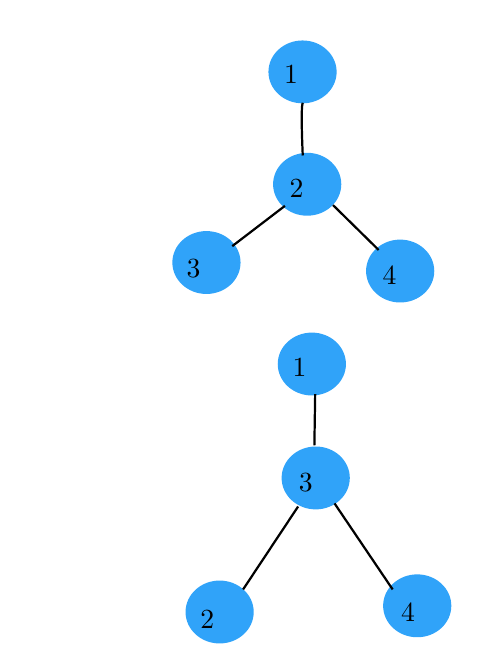
\begin{tikzpicture}[y=0.80pt,x=0.80pt,yscale=-1, inner sep=0pt, outer sep=0pt, scale = 0.35]
  \path[cm={{0.55,0.0,0.0,0.51636,(258.57143,453.83335)}},fill=c30a3f9]
    (285.7143,239.5050)arc(0.000:180.000:80.000000 and
    78.571)arc(-180.000:0.000:80.000000 and 78.571) -- cycle;
  \path[fill=black,line join=miter,line cap=butt,line width=0.800pt] (0,0)
    node[above right] (flowRoot4017) {};
  \path[cm={{0.55,0.0,0.0,0.51636,(134.57143,626.83335)}},fill=c30a3f9]
    (285.7143,239.5050)arc(0.000:180.000:80.000000 and
    78.571)arc(-180.000:0.000:80.000000 and 78.571) -- cycle;
  \path[cm={{0.55,0.0,0.0,0.51636,(253.57143,306.83335)}},fill=c30a3f9]
    (285.7143,239.5050)arc(0.000:180.000:80.000000 and
    78.571)arc(-180.000:0.000:80.000000 and 78.571) -- cycle;
  \path[cm={{0.55,0.0,0.0,0.51636,(241.57143,-70.16665)}},fill=c30a3f9]
    (285.7143,239.5050)arc(0.000:180.000:80.000000 and
    78.571)arc(-180.000:0.000:80.000000 and 78.571) -- cycle;
  \path[cm={{0.55,0.0,0.0,0.51636,(389.57143,618.83335)}},fill=c30a3f9]
    (285.7143,239.5050)arc(0.000:180.000:80.000000 and
    78.571)arc(-180.000:0.000:80.000000 and 78.571) -- cycle;
  \path[cm={{0.55,0.0,0.0,0.51636,(367.57143,186.83335)}},fill=c30a3f9]
    (285.7143,239.5050)arc(0.000:180.000:80.000000 and
    78.571)arc(-180.000:0.000:80.000000 and 78.571) -- cycle;
  \path[cm={{0.55,0.0,0.0,0.51636,(247.57143,74.83335)}},fill=c30a3f9]
    (285.7143,239.5050)arc(0.000:180.000:80.000000 and
    78.571)arc(-180.000:0.000:80.000000 and 78.571) -- cycle;
  \path[cm={{0.55,0.0,0.0,0.51636,(117.57143,175.83335)}},fill=c30a3f9]
    (285.7143,239.5050)arc(0.000:180.000:80.000000 and
    78.571)arc(-180.000:0.000:80.000000 and 78.571) -- cycle;
  \path[draw=black,line join=miter,line cap=butt,line width=0.800pt]
    (355.0000,93.3622) .. controls (352.0000,99.3622) and (355.0000,161.3622) ..
    (355.0000,161.3622);
  \path[draw=black,line join=miter,line cap=butt,line width=0.800pt]
    (264.0000,278.3622) -- (332.0000,226.3622);
  \path[draw=black,line join=miter,line cap=butt,line width=0.800pt]
    (394.0000,225.3622) -- (453.0000,283.3622);
  \path[draw=black,line join=miter,line cap=butt,line width=0.800pt]
    (371.0000,469.3622) -- (370.0000,535.3622);
  \path[draw=black,line join=miter,line cap=butt,line width=0.800pt]
    (396.0000,610.3622) -- (471.0000,721.3622);
  \path[draw=black,line join=miter,line cap=butt,line width=0.800pt]
    (278.0000,721.3622) -- (349.0000,614.3622);
  \path[fill=black,line join=miter,line cap=butt,line width=0.800pt] (0,0)
    node[above right] (flowRoot3264) {};
  \path[fill=black] (482,763.36218) node[above right] (text3272) {4};
  \path[fill=black] (223,772.36218) node[above right] (text3276) {2};
  \path[fill=black] (350,595.36218) node[above right] (text3280) {3};
  \path[fill=black] (342,446.36218) node[above right] (text3284) {1};
  \path[fill=black] (458,328.36218) node[above right] (text3288) {4};
  \path[fill=black] (205,318.36218) node[above right] (text3292) {3};
  \path[fill=black] (338,215.36218) node[above right] (text3296) {2};
  \path[fill=black] (331,68.362183) node[above right] (text3300) {1};

\end{tikzpicture}
\caption{The top tree, $T$, is a RRT on $n$ vertices. The bottom tree, $(2,3) \cdot T$ is obviously not a RRT.}\label{fig:1}
\end{figure}


\begin{remk}
Let $T \in \T_n$ correspond to $f \in \mathcal{F}_n$ then $\sigma \cdot T$ corresponds to the following  function:
\[ f'= \left(\begin{array}{cccccc}
     1& \sigma(2)&\sigma(3) &\sigma(4)& \dots & \sigma(n) \\
     1 & \sigma(f(2)) &\sigma(f(3)) &\sigma(f(4)) &\dots & \sigma(f(n))
    \end{array} \right)
\]

Let $T' = \sigma \cdot T$, there exists some function $g$ corresponding to $T'$ such that:
 \[ g= \left(\begin{array}{cccccc}
     1& \sigma(2)&\sigma(3) &\sigma(4)& \dots & \sigma(n) \\
     1 & g(\sigma(2)) &g(\sigma(3)) &g(\sigma(4)) &\dots & g(\sigma(n))
    \end{array} \right)
\]

Where $g(\sigma(i))$ is the father of $\sigma(i)$ but it is clear that the father of $\sigma(i)$ is $\sigma(f(i))$  hence $g(i) = \sigma(f(i))$ for $i = 2,3,\dots,n$.  
\end{remk}

\begin{corol}\label{cor:sig}
Let $T \in \T_n$ and $ \sigma \in S_n$.  Then  $\sigma  \cdot T \in \T_n$ if and only if $\sigma(f(i)) < \sigma(i) $. 
\end{corol}

\begin{remk}\label{remk:a} If $i$ and $j$ are adjacent vertices in a RRT, $T$, and $T$ is acted upon by the transposition $(i,j)$ then
 $\sigma \cdot T \notin \T_n$.  Without loss of generality assume that $i <j $.  Since $i$ and $j$ are adjacent $f(j) = i$, hence:
\[ \sigma(j) = i  < j = \sigma(i) =  \sigma(f(j))\]
The result follows from Corollary \ref{cor:sig}. 
\end{remk}

We define an indicator function for any $\sigma \in S_n$  and $ T \in \T_n$ as follows:
 \[ I(\sigma,T) = \left\{
  \begin{array}{l l}
    1 & \quad \text{if $\sigma \cdot T \in \T_n$}\\
    0 & \quad \text{otherwise}
  \end{array} \right.\]

\subsection{Transpositions}
In order to understand the effect of a permutation of vertices of a RRT we shall examine $\sigma \cdot T$ where $\sigma = (p,q)$ is a transposition.

By Corollary \ref{cor:sig} if $\sigma \cdot T \in T_n$ the corresponding function, $f$, satisfies $\sigma(f(i)) < \sigma(i)$ for $i = 2,3,\dots,n$.  

\begin{lem}\label{lem:rrtperm}
Given a RRT $T = \{T_{i}\}_{i=1}^{n}$ and a transposition $\sigma  = (p,q)$ such that $p <q$, the labelled tree $\sigma  \cdot T$ is a RRT if and only if $f(q)< p$ and $p$ is a leaf in $T_q$ .   
\end{lem}
\begin{remk}\label{remk:split}
The proof of  Lemma \ref{lem:rrtperm} relies on the fact that that any  $f \in \mathcal{F}_n$  can be split up into 5 parts as follows:
 \[ f = \left(\begin{array}{ccc|c|ccc|c|ccc}
     1    & \dots & p-1    &   p  & p+1    & \dots & q-1    & q    & q+1    & \dots & n \\
     f(1) & \dots & f(p-1) & f(p) & f(p+1) & \dots & f(q-1) & f(q) & f(q+1) & \dots & f(n)
    \end{array} \right)
\]

Notice that the first and fifth parts (with domain $i < p$ and $i > q$ respectively) are irrelevant to whether or not $\sigma \cdot T$ is a random recursive tree.  It remains to find necessary and sufficient conditions for the second third and fourth parts such that $\sigma \cdot T \in \T_n$.   

\end{remk}
\begin{proof}{[of Lemma \ref{lem:rrtperm}]}  
Let $f \in \F_n$ correspond to a RRT $T$.  We can partition the domain of $f$ into 5 sets as follows: 
\begin{case}[$i<p$]
Since $T$ is a RRT $f(i) < i < p$ therefore $\sigma(i) = i$ and $\sigma(f(i))$ = $f(i)$ so we trivially have $\sigma(f(i)) < \sigma(i)$.
\end{case}
\begin{case}[$i=p$]
Since $T$ is a RRT $f(p) < p$ so $\sigma(f(p)) = f(p)$.  Therefore $\sigma(f(p)) = f(p) < p < q  = \sigma(p)$ is always satisfied.
\end{case}
\begin{case}[$p<i<q$]
 Since $i \neq p$ and $i \neq q$,  $\sigma(i) = i$. Also note that since $T$ is a RRT $f(i) < i < q$.  Therefore, $\sigma \cdot T \in \T_n$ if and only if $\sigma(f(i)) < i$ which is the case if and only if $f(i) \neq p$.   
\end{case}
\begin{case}[$i=q$]
 By Remark \ref{remk:a} if $f(q) = p$ then $\sigma \cdot T$ is \emph{not} an RRT.  
 Furthermore, $\sigma \cdot T$ is a RRT if and only if:
 \begin{align*}
  \sigma(f(q)) &< \sigma(q)  \\
  \iff \sigma(f(q)) &< p
 \end{align*}
This is the case if and only if $f(q) <p$.
\end{case}
\begin{case}[$i>q$]
Since $i \neq p$ and $i \neq q$ it is always the case that $\sigma(i) = i$ hence 
\[\sigma(f(i)) =
\left\{
  \begin{array}{l l}
    f(i) & \quad \text{if $f(i) \neq p,q$}\\
    p & \quad \text{if $f(i) = q$}\\
    q & \quad \text{if $f(i) = p$}
  \end{array} \right.\]
Since $f(i),p,q < i$ it is always the case that $\sigma(i) < \sigma(f(i))$.  
\end{case}
Therefore $\sigma \cdot T \in \T_n$ if and only if $f(q) < p $ \emph{and} $f(i) \neq p$ for $i = p+1,p+2,\dots,q-1$.  Equivalently we could say $\sigma \cdot T \in \T_n$ if and only if $f(q)< p$ and $p$ is a leaf in $T_q$. 
\end{proof}

%write something here.

\begin{lem}\label{lem:pn}
 Fix $ \sigma \in S_n$ and write $P_n(\sigma) = \sum_{T \in T_n}I(\sigma,T)$.  For any transposition $\sigma = (p,q)$ such that $p< q$:
 \[P_n(\sigma) = \frac{(p-1)^{2}}{(q-1)(q-2)}\] 
\end{lem}
\begin{proof}
Let $\sigma$ be as in the statement of Lemma \ref{lem:pn}. Note that $P_n(\sigma)$  is the number of trees $T \in \T_n$ such that $(p,q) \cdot T \in \T_n$. By Lemma \ref{lem:rrtperm},  $\sigma   \cdot T \in T_n$ if and only if $p$ is a leaf in $T_q$ and $f(q)< p$.  Therefore,  $P_n(\sigma)$ is the number of trees $T \in \T_n$ such that $p$ is a leaf in $T_q$ and $f(q)< p$.  

For every $T \in \T_n$ the associated function $f$ can be split up into 5 parts as described in Remark \ref{remk:split}. In particular the following matrix shows the number of possible values of $f(i)$ such that $\sigma \cdot T \in \T_n$:

 \[\left(\begin{array}{cccc|c|ccc|c|ccc}
     1  & 2  & 3 & \dots & p   & p+1 & \dots & q-1 & q    & q+1    & \dots & n \\
     1  & 1  & 2 & \dots & p-1 & p-1 & \dots & q-2 & p-1  & q      & \dots & n-1
    \end{array} \right)
\]
Therefore,  
\begin{align*}
 P_n(p,q) &= % 1 \times 2 \dots (i-1) \times (i-1) \times (i-1) \times \dots \times (j-2) \times (i-1) \times j \times (j-1) \times (n-1) \\
 \frac{(p-1)^2}{(q-1)(q-2)}(n-1)!
\end{align*}
\end{proof}



\section{$n$-cycles}
In this section we will generalise  Lemma \ref{lem:rrtperm} to permutations $\sigma = (p_1,p_2,\dots,p_m)$ such that $p_1 < p_2 < \dots < p_m $.  The proof of Lemma \ref{lem:mcycles} follows closely the proof of Lemma \ref{lem:rrtperm}.
\begin{lem}\label{lem:mcycles}
Given a RRT $T = \{T_{i}\}_{i=1}^{n}$ and a transposition $\sigma  = (p_1,p_2,\dots,p_m)$ the labelled tree $\sigma  \cdot T$ is a RRT if and only if  $f(p_m) < p_1$ \emph{and} wither $p_l$ is a leaf in $T_{l+1}$ \emph{or} $f(p_{l+1}) = f(p_l)$ for $l = 1,2,\dots m-1$.   
\end{lem}

\begin{proof}
Let $T \in \T_n$ be a RRT and $f \in \mathcal{F}_n$ be the corresponding function. Following the argument from the proof of Lemma \ref{lem:rrtperm} we can see immediately that there are no conditions on $f(i)$ for $i \leq p_1$ and $i > p_m$ for $\sigma \cdot T \in T_n$. 

For $p_l < i < p_{l+1}$, if $f(i) = p_l$ then $\sigma(i) = i$ and $\sigma(f(i)) = p_{l+1}$ for $l = 1,2,\dots, m-1$.  This means that:
\[\sigma(i) = i < p_{l+1}  = \sigma{f(i)},\]
which is the case if and only if $\sigma \cdot T$ is \emph{not} a RRT. For another value of $f(i)$ either $i \notin \sigma$ in which case $\sigma(f(i)) =  f(i) < i = \sigma(i)$ \emph{or} $i = p_k$ for some $1 \leq k <l$ so $\sigma(f(i)) = p_{k+1} \leq p_l < i = \sigma(i)$.   

We now need only consider $i = p_l$ for $l = 2,3,\dots,m$. By Corollary \ref{cor:sig} $\sigma \cdot T \in T_n$ if and only if $\sigma(f(i)) < p_{l+1}  = \sigma{f(i)}$ for  $l = 1,2,\dots, n-1$, this is clearly always satisfied.  Bo Corrolary \ref{cor:sig} $\sigma \cdot T \in T_n$ if and only if
\[ \sigma(f(i)) < \sigma(i) = p_{l+1}.\]
Since $f(i) < p_l$ this condition is trivially satisfied. 


Finally, consider $p_m$.  Note that if $\sigma \cdot T \in \T_n$ if and only if 
\[\sigma(f(p_m)) < \sigma(p_m) = p_1\]
In conclusion, $\sigma \cdot T \in \T_n$ if and only if $f(p_m) < p_1$.  

\end{proof}
\begin{corol}
  Let $\sigma \in S_n$ have the form $\sigma = (p_1,p_2,p_3,\dots p_m)$ such that $p_1 < p_2 < \dots < p_m$.  
  
  \[P_n(\sigma) = \frac{(p_1-1)^{2}(p_2 -1)(p_3-1)\dots(p_m -1)}{(p_2 - 2)(p_3 - 2)\dots(p_m-2)(p_m-1)} (n-1)!.\] 

  \end{corol}
\begin{proof}
 We use a similar method to the proof of Lemma \ref{lem:pn}.  Recall that we can think of $P_n(\sigma)$  as the number of trees $T \in \T_n$ such that $\sigma \cdot T \in \T_n$. By Lemma \ref{lem:mcycles}, given a RRT $\{T = T_{i}\}_{i=1}^{n}$ and a transposition $\sigma  = (p_1,p_2,\dots,p_m)$ the labelled tree $\sigma  \cdot T$ is a RRT if and only if  $p_l$ is a leaf in $T_{p_{l+1}}$ for $l = 1,2,\dots,n-1$ and $f(p_m) < p_1$.  

We therefore know the number of possible values that $f(i)$ can take for each $i$. The following matrix shows the number of possible values of $f(i)$ for $p_1 < i < p_m$. 

 \[\left(\begin{array}{ccccccccccc}
     \dots & p_1      & p_1 +1   & \dots & p_2 - 1 & p_2   & p_2 + 1 & \dots & p_m - 1 & p_m & \dots \\
     \dots & p_1 - 1  & p_1 - 1  & \dots & p_2 - 3 & p_2-1 & p_2-1   & \dots & p_m-3   & p_1-1 & \dots  
    \end{array} \right)
\]
\end{proof}
 
\begin{remk}
Let $T \in T_n$ and a permutation $ \sigma  = (p_1,p_2,\dots,p_m)$ such that $p_1 < p_2 < \dots p_m$ and denote transpositions $\sigma_l = (p_1,p_l)$ for $l = 1,2,\dots,m$.
%Do those transpositions generate \sigma ?
It is interesting to note that given a random recursive tree $T$ such that $\sigma \cdot T \in \T_n$ it is \emph{not} necessarily the case that $\sigma_l \cdot T \in T_n$.  If we let $T$ be the RRT given in Figure  \ref{fig:int} it is clear that $(234) \cdot T \in \T_4$ but $(23) \cdot T \notin \T_4 $.   
 
 \begin{figure}[h]
 \centering
 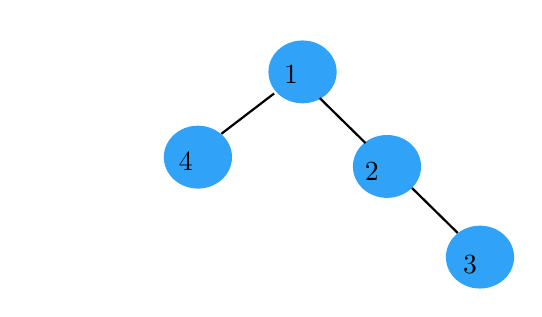
\begin{tikzpicture}[y=0.80pt,x=0.80pt,yscale=-1, inner sep=0pt, outer sep=0pt, scale = 0.35]
  \path[fill=black,line join=miter,line cap=butt,line width=0.800pt] (0,0)
    node[above right] (flowRoot4017) {};
  \path[cm={{0.55,0.0,0.0,0.51636,(241.57143,-70.16665)}},fill=c30a3f9]
    (285.7143,239.5050)arc(0.000:180.000:80.000000 and
    78.571)arc(-180.000:0.000:80.000000 and 78.571) -- cycle;
  \path[cm={{0.55,0.0,0.0,0.51636,(106.57143,39.83335)}},fill=c30a3f9]
    (285.7143,239.5050)arc(0.000:180.000:80.000000 and
    78.571)arc(-180.000:0.000:80.000000 and 78.571) -- cycle;
  \path[cm={{0.55,0.0,0.0,0.51636,(350.57143,51.83335)}},fill=c30a3f9]
    (285.7143,239.5050)arc(0.000:180.000:80.000000 and
    78.571)arc(-180.000:0.000:80.000000 and 78.571) -- cycle;
  \path[cm={{0.55,0.0,0.0,0.51636,(470.57143,168.83335)}},fill=c30a3f9]
    (285.7143,239.5050)arc(0.000:180.000:80.000000 and
    78.571)arc(-180.000:0.000:80.000000 and 78.571) -- cycle;
  \path[draw=black,line join=miter,line cap=butt,line width=0.800pt]
    (250.0000,133.3622) -- (318.0000,81.3622);
  \path[draw=black,line join=miter,line cap=butt,line width=0.800pt]
    (496.0000,203.3622) -- (555.0000,261.3622);
  \path[fill=black,line join=miter,line cap=butt,line width=0.800pt] (0,0)
    node[above right] (flowRoot3264) {};
  \path[fill=black] (195,181.36218) node[above right] (text3288) {4};
  \path[fill=black] (562,313.36218) node[above right] (text3292) {3};
  \path[fill=black] (435,193.36218) node[above right] (text3296) {2};
  \path[fill=black] (331,68.362183) node[above right] (text3300) {1};
  \path[draw=black,line join=miter,line cap=butt,line width=0.800pt]
    (377.0000,87.3622) -- (436.0000,145.3622);

\end{tikzpicture}
 \caption{}\label{fig:int}
 \end{figure}
\end{remk}
 
 We can make the following corollary.  


\begin{corol}\label{cor:subsig}
 Let $T \in T_n$ and a permutation $ \sigma  = (p_1,p_2,\dots,p_m)$ such that $p_1 < p_2 < \dots <  p_m$ and $\sigma \cdot T \in \T_n$.  Let $\sigma^{(l)} = (p_l,p_l+1,\dots,p_m)$, then $\sigma' \cdot T \in \T_n$ for $l = 1,2,\dots m-1$.
\end{corol}
\begin{proof}
 Assume that $T$ and $\sigma$ are as in the statement of this corollary and consider $\sigma^{l} \cdot T$.  By Lemma \ref{lem:mcycles} $f(p_m) < p_1 < p_l$ and either $(p_i)$ is a leaf in $T_{i+1}$ for $i = l,l+1,\dots,m$.       
\end{proof}

\begin{remk}
 The converse of Corollary \ref{cor:subsig} is not true.  %add example.   %take Figure \ref{fig:int} for example.
\end{remk}

\section{Enumeration of legal moves part 2}
In this section we will calculate $Q_n = \sum_{\sigma \in S_n}\sum_{T \in \T_n}$ for certain specific cases of $\sigma$ beginning with transpositions.  We can write out all transpositions $(p,q) \in S_n$ in a grid form as follows:
 \[ \begin{array}{c|c|c|c|c}
     (2,3)  & (2,4)  & (2,5) & \dots & (2,n) \\
       & (3,4)  & (3,5) & \dots &(3,n) \\
       &        &  (4,5) & \dots & (4,n) \\
       &&&& \vdots \\
       &&&&(n-1,n)
    \end{array} 
\]
By Lemma \ref{lem:pn}, for any transposition $\sigma(p,q)$ 
\[P_n = \lvert \T_n\rvert\frac{(p-1)^{2}}{(q-1)(q-2)}\]
To calculate $Q_n$ we simply sum $P_n$ over the columns of the grid above:  
\begin{align*}
 Q_{n} &= \lvert \T_n\rvert\sum_{i=1}^{n-2} \left( \frac{ \sum_{j=1}^{i} j^2}{i(i+1)} \right) \\
 &= \lvert \T_n\rvert\frac{1}{6} \sum_{i=1}^{n-2} \frac{i(i+1)(2i +1)}{i(i+1)}\\
 &= \lvert \T_n\rvert\frac{1}{6} \sum_{i=1}^{n-2} 2i +1 \\
 & = \frac{\lvert \T_n\rvert}{6} n(n-2) 
\end{align*}

\section{Notation}
\begin{itemize}
 \item[$\{T_i\}_{i=1}^{n}$] A random recursive tree process on $n$ vertices.
 \item[$\T_n$] The set of of random recursive tree processes on $n$ vertices.
 \item[$\tilde{\T}_n$] The set of labelled rooted tree on $n$ vertices.
 \item[$S_n$]  the symmetric group on $n$ elements.
 \item[ $ I(\sigma,T)$] $$ \left\{
  \begin{array}{l l}
    1 & \quad \text{if $\sigma \cdot T \in \T_n$}\\
    0 & \quad \text{otherwise}
  \end{array} \right.$$
  \item[$P_n(\sigma)$] $ \sum_{T \in T_n}I(\sigma,T)$
  \item[$Q_n$]  $\sum_{\sigma \in S_n}\sum_{T \in \T_n}$
\end{itemize}


\end{document}
